\documentclass[11pt]{article}

\usepackage{latexsym}
\usepackage{algorithm,algpseudocode}
\usepackage{amsmath}
\usepackage{amssymb}
\usepackage{amsthm}
\usepackage{graphicx}
\usepackage{wrapfig}
\usepackage{pseudocode}
\usepackage{subfigure}
\usepackage{url}
\usepackage[backref, colorlinks=true, citecolor=red, urlcolor=blue, pdfauthor={Jyh-Ming Lien}]{hyperref}


\newcommand{\handout}[5]{
  \noindent
  \begin{center}
  \framebox{
    \vbox{
      \hbox to 5.78in { {\bf } \hfill #2 }
      \vspace{4mm}
      \hbox to 5.78in { {\Large \hfill #5  \hfill} }
      \vspace{2mm}
      \hbox to 5.78in { {\em #3 \hfill #4} }
    }
  }
  \end{center}
  \vspace*{4mm}
}

\newcommand{\lecture}[4]{\handout{#1}{#2}{#3}{#4}{#1}}

\newtheorem{theorem}{Theorem}
\newtheorem{corollary}[theorem]{Corollary}
\newtheorem{lemma}[theorem]{Lemma}
\newtheorem{observation}[theorem]{Observation}
\newtheorem{proposition}[theorem]{Proposition}
\newtheorem{definition}[theorem]{Definition}
\newtheorem{claim}[theorem]{Claim}
\newtheorem{fact}[theorem]{Fact}
\newtheorem{assumption}[theorem]{Assumption}

% 1-inch margins, from fullpage.sty by H.Partl, Version 2, Dec. 15, 1988.
\topmargin 0pt
\advance \topmargin by -\headheight
\advance \topmargin by -\headsep
\textheight 8.9in
\oddsidemargin 0pt
\evensidemargin \oddsidemargin
\marginparwidth 0.5in
\textwidth 6.5in

\parindent 0in
\parskip 1.5ex
%\renewcommand{\baselinestretch}{1.25}

\begin{document}

\lecture{Midterm Exam Report}{Fall 2015}{Yeojin Kim}{Advance Algorithm Programming}

\section{Summary of the two methods}
  Both hedcuter method and voronoi method repeat two steps : constructing weighted voronoi diagram and moving sites to new centroids. %% convergence
\subsection{hedcuter method}
%%The idea of hedcuter method
%%Flow
%%Sampling
Before constructing weighted voronoi diagram, the method samples the entire image pixel space. Using uniform 
%%CVT & moving sites
To construct weighted voronoi diagram, the method adopts centroid voronoi tessellation. 
%%Creating disks

\subsection{voronoi method}
%%Idea
%%Flow
%%Sampling
%%Voronoi diagram & moving sites
%%Creating disks

\section{Improvement of hedcuter method}
%size
\begin{figure*}[hbt]
 \centering
 \subfigure[]{
    \includegraphics[width=0.22\textwidth]{FIGS/size/cat-xsmall.png}
    \label{fig:cat_xs}
  }\hspace{-3mm}
  \subfigure[]{
    \includegraphics[width=0.22\textwidth]{FIGS/size/cat-small.png}
    \label{fig:cat_s}
  }\hspace{-3mm}
  \subfigure[]{
    \includegraphics[width=0.22\textwidth]{FIGS/size/cat-middle.png}
    \label{fig:cat_s}
  }\hspace{-3mm}
  \subfigure[]{
    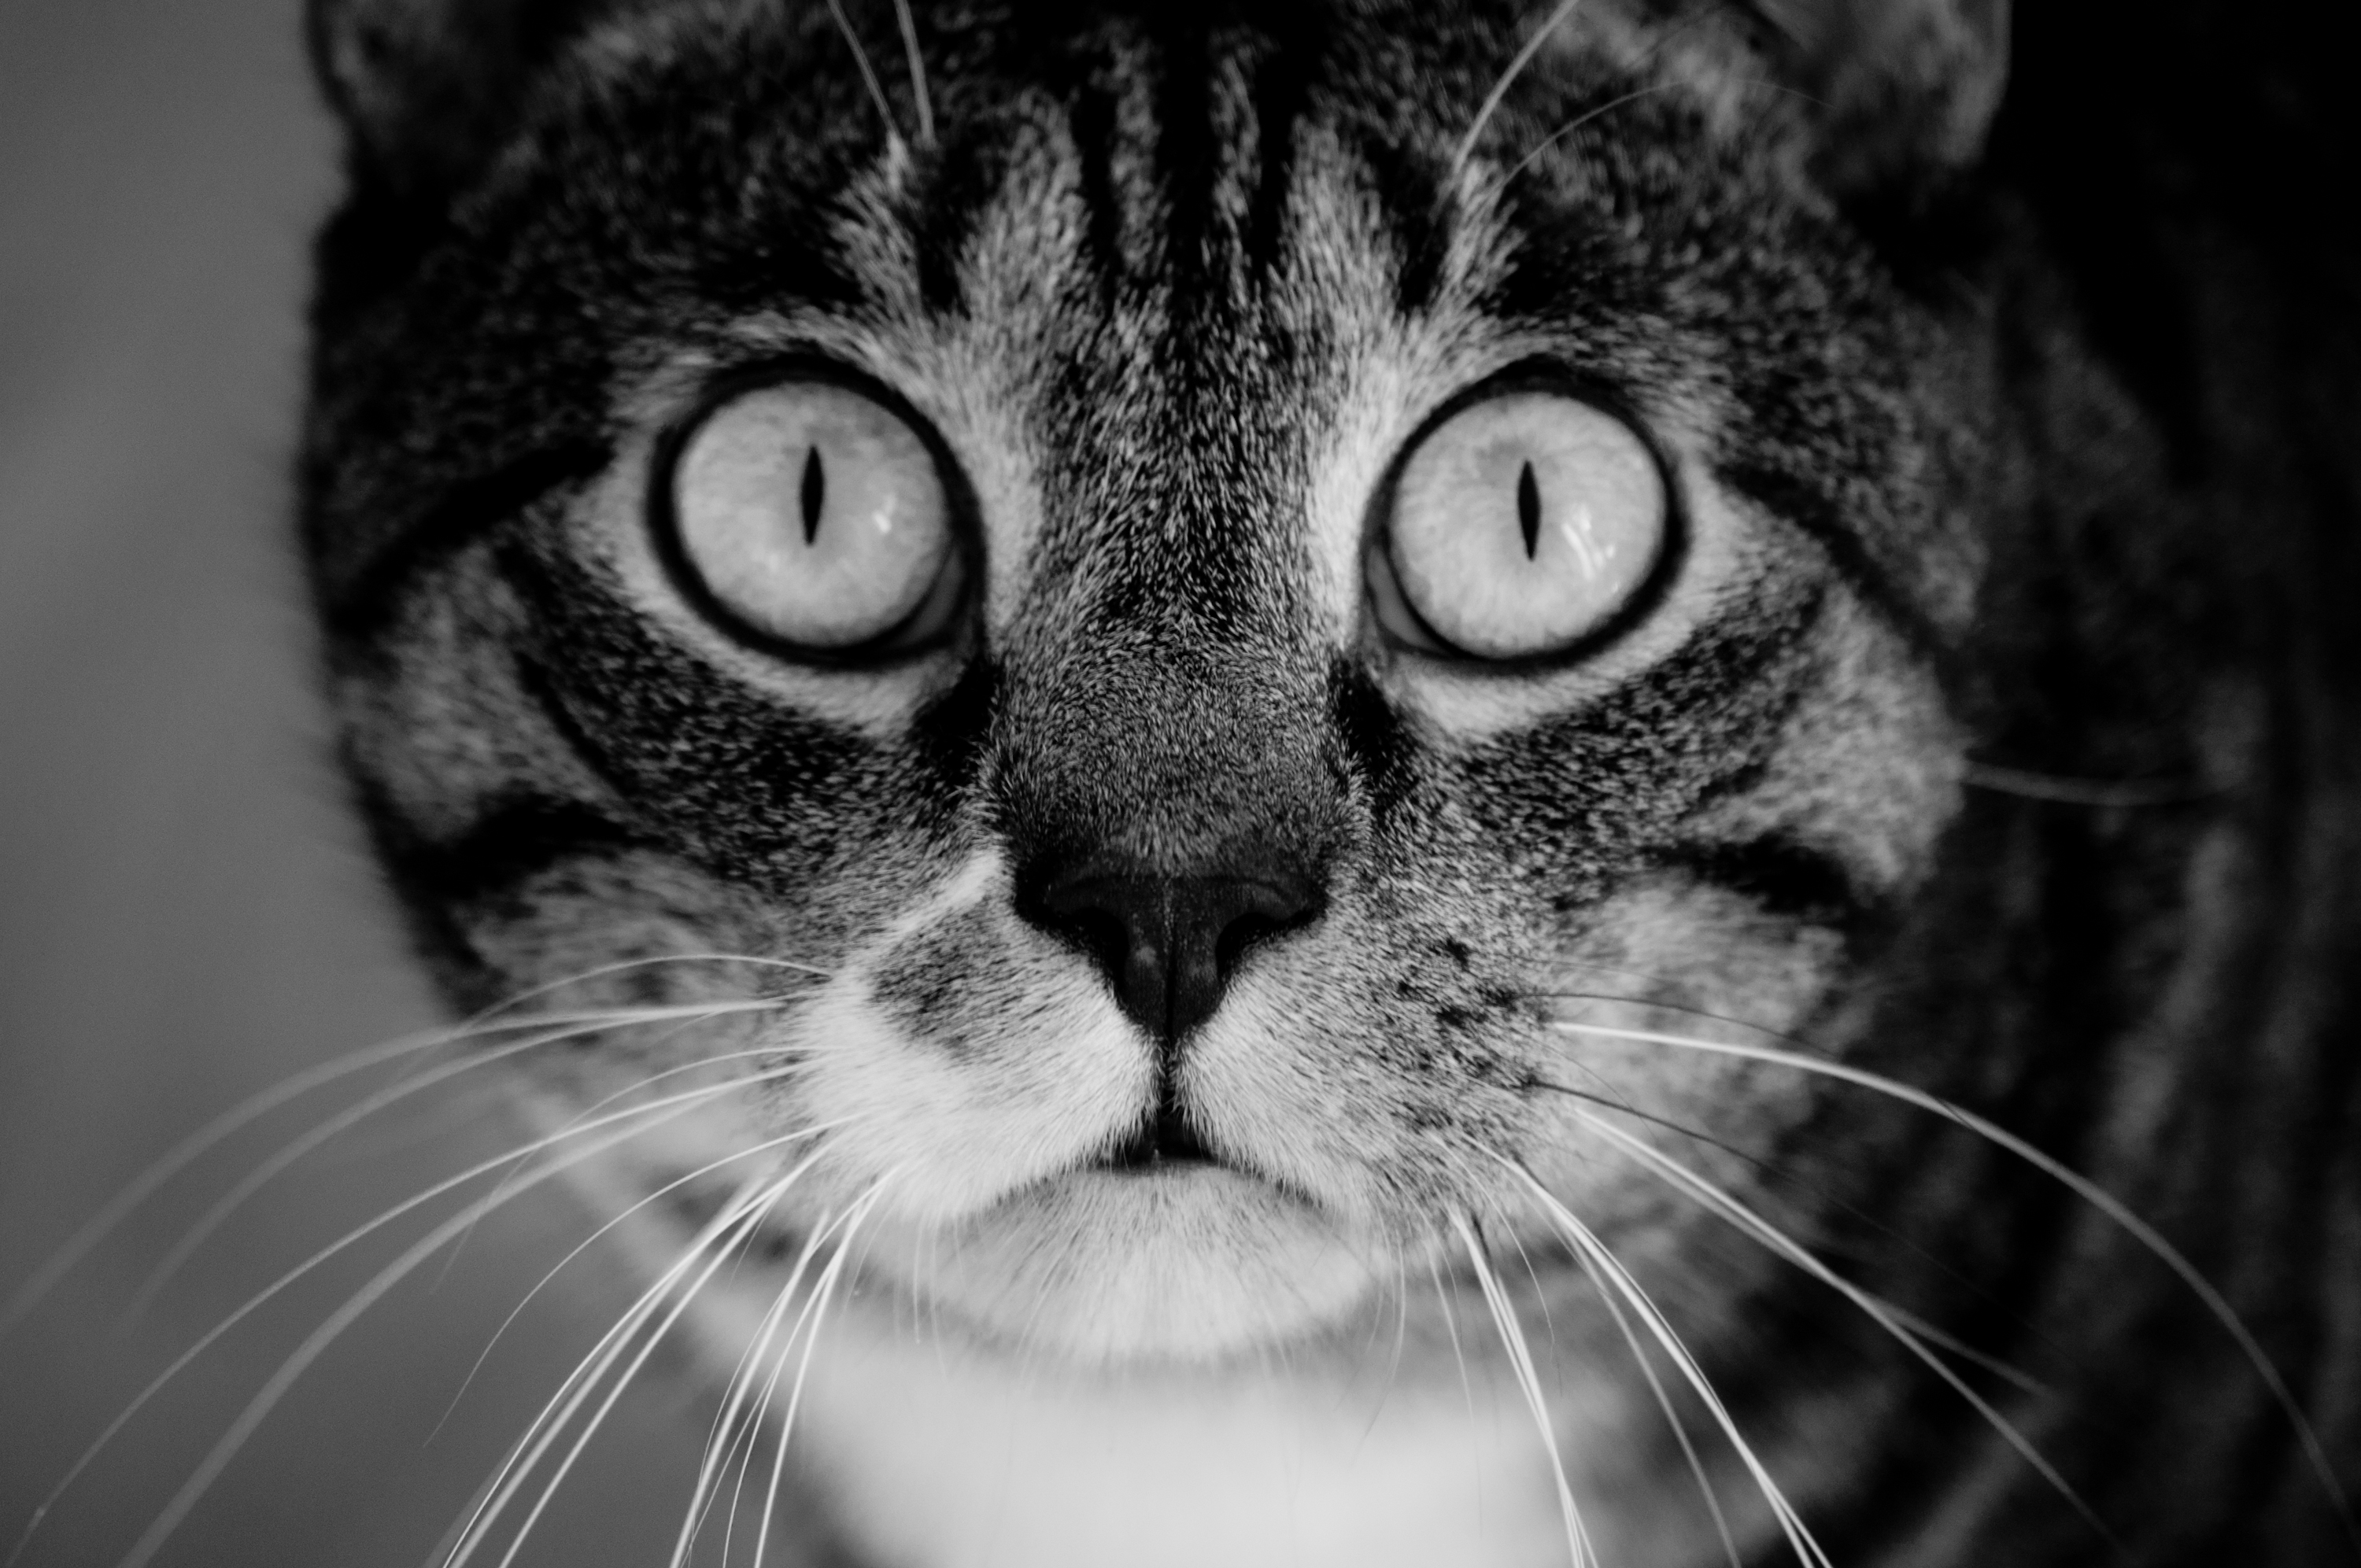
\includegraphics[width=0.22\textwidth]{FIGS/size/cat-large.png}
    \label{fig:cat_s}
  }\hspace{-3mm}
    \caption{A part of given image and sample points. \label{fig:cat_size}}
\end{figure*}
%Brightness
\begin{figure*}[hbt]
 \centering
 \subfigure[]{
    \includegraphics[width=0.22\textwidth]{FIGS/brightness/cat-b-40.png}
    \label{fig:cat_b-40}
  }\hspace{-3mm}
  \subfigure[]{
    \includegraphics[width=0.22\textwidth]{FIGS/brightness/cat-b-20.png}
    \label{fig:cat_b-20}
  }\hspace{-3mm}
  \subfigure[]{
    \includegraphics[width=0.22\textwidth]{FIGS/brightness/cat-b+20.png}
    \label{fig:cat_b+20}
  }\hspace{-3mm}
  \subfigure[]{
    \includegraphics[width=0.22\textwidth]{FIGS/brightness/cat-b+40.png}
    \label{fig:cat_b+40}
  }\hspace{-3mm}
    \caption{A part of given image and sample points. \label{fig:cat_brightness}}
\end{figure*}
%Contrast
\begin{figure*}[hbt]
 \centering
 \subfigure[]{
    \includegraphics[width=0.22\textwidth]{FIGS/contrast/cat-c-40.png}
    \label{fig:cat_c-40}
  }\hspace{-3mm}
  \subfigure[]{
    \includegraphics[width=0.22\textwidth]{FIGS/contrast/cat-c-20.png}
    \label{fig:cat_c-20}
  }\hspace{-3mm}
  \subfigure[]{
    \includegraphics[width=0.22\textwidth]{FIGS/contrast/cat-c+20.png}
    \label{fig:cat_c+20}
  }\hspace{-3mm}
  \subfigure[]{
    \includegraphics[width=0.22\textwidth]{FIGS/contrast/cat-c+40.png}
    \label{fig:cat_c+40}
  }\hspace{-3mm}
    \caption{A part of given image and sample points. \label{fig:cat_contrast}}
\end{figure*}
%sharpness
\begin{figure*}[hbt]
 \centering
 \subfigure[]{
    \includegraphics[width=0.22\textwidth]{FIGS/sharpness/cat-s-50.png}
    \label{fig:cat_s-40}
  }\hspace{-3mm}
  \subfigure[]{
    \includegraphics[width=0.22\textwidth]{FIGS/sharpness/cat-s-25.png}
    \label{fig:cat_s-20}
  }\hspace{-3mm}
  \subfigure[]{
    \includegraphics[width=0.22\textwidth]{FIGS/sharpness/cat-s+25.png}
    \label{fig:cat_s+20}
  }\hspace{-3mm}
  \subfigure[]{
    \includegraphics[width=0.22\textwidth]{FIGS/sharpness/cat-s+50.png}
    \label{fig:cat_s+40}
  }\hspace{-3mm}
    \caption{A part of given image and sample points. \label{fig:cat_sharpness}}
\end{figure*}
\bibliographystyle{plain}
\bibliography{report}

\end{document}


